% ======================================================================
% Software Requirement Specification (SRS) — AutoCompose
% MCA 3rd Semester Mini Project
%
% NOTES FOR THE STUDENT (delete this comment block before submission):
%  - Search for "[FILL:" throughout this file and replace every such
%    placeholder with your actual details (names, roll numbers, guide
%    name, batch, client name, institution-specific figures).
%  - Compile with pdflatex, TWICE (so the Table of Contents resolves
%    page numbers correctly):
%        pdflatex srs_autocompose.tex
%        pdflatex srs_autocompose.tex
%  - The body font below is set with `mathptmx`, which substitutes a
%    Times-metric-compatible font under pdfLaTeX. If your department
%    insists on literal "Times New Roman" (the .ttf), recompile with
%    xelatex/lualatex and replace the mathptmx line with:
%        \usepackage{fontspec}\setmainfont{Times New Roman}
%  - "UCC- MCA" in the footer is taken verbatim from the format sheet;
%    replace it if your institution's footer text differs.
% ======================================================================

\documentclass[12pt,a4paper]{article}

% ---------- Core packages ----------
\usepackage[utf8]{inputenc}
\usepackage[T1]{fontenc}
\usepackage{mathptmx}                 % Times-compatible font for pdfLaTeX
\usepackage[a4paper,left=1in,right=1in,top=1.3in,bottom=1.2in,%
            headheight=26pt,headsep=16pt,footskip=28pt]{geometry}
\usepackage{titlesec}
\usepackage{fancyhdr}
\usepackage{eso-pic}
\usepackage{tikz}
\usetikzlibrary{calc,positioning}
\usepackage{enumitem}
\usepackage{array}
\usepackage{tabularx}
\usepackage{booktabs}
\usepackage{caption}
\usepackage{graphicx}
\usepackage[hidelinks]{hyperref}

% ---------- Project identity (edit once, used everywhere) ----------
\newcommand{\ProjectTitle}{AUTOCOMPOSE -- AI EMAIL ASSISTANT}
% [FILL: replace the line above with your officially approved project
%  title if it differs from the one used throughout this draft.]

% ---------- Page border on every page ----------
\AddToShipoutPictureBG{%
  \begin{tikzpicture}[remember picture,overlay]
    \draw[black,line width=1pt]
      ($(current page.north west)+(0.5in,-0.5in)$) rectangle
      ($(current page.south east)+(-0.5in,0.5in)$);
  \end{tikzpicture}%
}

% ---------- Header / Footer (applied to every page) ----------
\pagestyle{fancy}
\fancyhf{}
\renewcommand{\headrulewidth}{0.6pt}
\renewcommand{\footrulewidth}{0.6pt}
\fancyhead[L]{\fontsize{10}{12}\selectfont \ProjectTitle}
\fancyhead[R]{\fontsize{10}{12}\selectfont SRS}
\fancyfoot[L]{\fontsize{10}{12}\selectfont UCC- MCA}
\fancyfoot[R]{\fontsize{10}{12}\selectfont \thepage}

% ---------- Heading styles ----------
% Section headings: 14pt, bold, UPPER CASE
\titleformat{\section}
  {\bfseries\fontsize{14}{17}\selectfont}{\thesection.}{0.6em}{\MakeUppercase}
\titlespacing{\section}{0pt}{1.4em}{0.8em}

% Subsection headings: 12pt, bold, Title Case
\titleformat{\subsection}
  {\bfseries\fontsize{12}{15}\selectfont}{\thesubsection.}{0.6em}{}
\titlespacing{\subsection}{0pt}{1.0em}{0.5em}

% Sub-subsection headings: 12pt, bold, Title Case (one level deeper, e.g. 12.4.1)
\titleformat{\subsubsection}
  {\bfseries\fontsize{12}{15}\selectfont}{\thesubsubsection.}{0.6em}{}
\titlespacing{\subsubsection}{0pt}{0.8em}{0.4em}

% Captions: "Figure 1: ..." / "Table 1: ..." with bold label
\captionsetup{labelfont=bf,labelsep=colon,font={normalsize}}

% Regular body text stays at the document's base size (12pt, normal) —
% no further changes needed since \documentclass[12pt]{article} already
% sets \normalsize to 12pt.

\setlength{\parindent}{18pt}

\begin{document}

% ======================================================================
% FRONT PAGE
% ======================================================================
\begin{titlepage}
\centering
\vspace*{1.2cm}

{\fontsize{14}{17}\selectfont\bfseries MINI PROJECT}\\[2.2cm]

{\fontsize{20}{24}\selectfont\bfseries \ProjectTitle}\\[1.4cm]

{\fontsize{16}{19}\selectfont\bfseries SOFTWARE REQUIREMENT SPECIFICATION (SRS)}\\[2.4cm]

\begin{flushleft}
\fontsize{12}{16}\selectfont
\textbf{Group Member Names:}\\[0.3cm]
1. \quad ALBY A B, \quad Roll No.\ 11\\
2. \quad FIDHA PARVIN , \quad Roll No.\ 31\\
% [FILL: duplicate the line above as "3. Name, Roll No." if your
%  group has a third member.]
\vspace{0.9cm}

\textbf{Guide:} Dr. Greeshma KV\\[0.5cm]
\textbf{Batch:} 3B\\[0.5cm]
\textbf{Client Name (if any):}  Public Platform for Students and Professionals
\end{flushleft}

\end{titlepage}

% ======================================================================
% TABLE OF CONTENTS
% ======================================================================
\tableofcontents
\newpage

% ======================================================================
% 1. INTRODUCTION
% ======================================================================
\section{Introduction}

This document presents the Software Requirement Specification (SRS) for the project \textbf{AutoCompose}, developed as part of the Master of Computer Applications (MCA) Mini Project for the third semester. The purpose of this document is to provide a comprehensive description of the system requirements, design considerations, and functional scope of the application. It serves as a common reference for the project guide, evaluators, and development team to understand the objectives, features, and implementation approach of the system.

AutoCompose is an AI-powered web application designed to assist users in drafting, managing, scheduling, and sending professional emails efficiently. The system utilizes large language models to generate email content based on user prompts and personalized profile information. Generated emails can be reviewed, edited, and delivered through the user's Gmail account either immediately or at a scheduled date and time, and, for users who prefer chat-based access, through an integrated Telegram bot.

The application aims to reduce the time and effort required for professional email communication while improving the quality, consistency, and effectiveness of email content. By integrating artificial intelligence with modern web technologies, AutoCompose provides an intelligent and user-friendly platform for email automation and communication management.

The subsequent sections of this document discuss the problem statement, proposed solution, feasibility analysis, system architecture, technology stack, and the detailed functional and non-functional requirements implemented in the current version of the system.




% ======================================================================
% 2. PROBLEM STATEMENT
% ======================================================================
\section{Problem Statement}

Professional email writing is a common yet time-consuming task for students, job seekers, and working professionals. Preparing emails such as leave requests, job applications, complaints, follow-ups, and formal inquiries requires appropriate language, structure, and tone. Many users, particularly those who are not confident in formal English communication, find it difficult to compose effective and professionally written emails.

Although general-purpose AI chat assistants can generate email content, they are not specifically designed for end-to-end email management workflows. Users often need to repeatedly provide their personal and professional information in every conversation. Additionally, these platforms do not maintain organized records of previously generated emails, making it difficult to revisit or reuse earlier drafts. Creating multiple emails for different recipients requires repetitive prompting, which reduces productivity and increases effort.

Furthermore, generated content must usually be copied manually into external email clients before it can be sent. Most AI chat systems also lack features such as email scheduling, batch generation, and integrated delivery mechanisms, resulting in a fragmented workflow.

AutoCompose addresses these limitations by providing an AI-powered email composition platform that combines intelligent content generation with user profile management, session-based history, batch email generation, direct Gmail integration, email scheduling capabilities, and a Telegram bot for composing and sending emails on the move. The system allows users to generate, manage, send, and schedule professional emails within a single application, thereby reducing effort, improving writing quality, and streamlining the entire email communication process.


% ======================================================================
% 3. SCOPE AND RELEVANCE OF THE PROJECT
% ======================================================================
\section{Scope and Relevance of the Project}

The system covers six areas:
\begin{enumerate}[leftmargin=22pt]
  \item AI-assisted generation of email drafts, individually or in batches, from a free-text prompt, a category, and an optional tone.
  \item Persistent storage and retrieval of past drafts and conversations, organised into single and batch sessions, with rename, archive, search, soft-delete, and a bulk ``Clear All Sessions'' action.
  \item A user profile that supplies personal, professional, and stylistic context to the AI, including resume-derived data used for job-application emails, with a dedicated editor for reviewing and correcting the AI-parsed resume fields.
  \item Delivery of the finished draft through the user's own Gmail account using an application-specific password, with the credential encrypted at rest, including optional file attachments.
  \item Deferred delivery of a drafted email through user-defined schedules, processed automatically by a background worker or cron job at the scheduled date and time.
  \item A companion Telegram bot that lets a linked user compose, review, regenerate, and send a single email entirely from a chat interface, using the same profile, AI models, and Gmail delivery path as the web application.
\end{enumerate}

The following are explicitly \textbf{not} in scope for the current version of the system: integration with corporate mail servers or any provider other than Gmail; offline use; real-time collaborative editing of a single draft by more than one user simultaneously; migration of a user's pre-existing email history from another platform; batch composition from within Telegram (the bot currently supports single-email composition only); and a dedicated native mobile application. The primary interface remains a responsive web application, with the Telegram bot serving as a lightweight, chat-based channel for on-the-go use rather than a full native app. One-time environment setup -- provisioning the MongoDB Atlas cluster, obtaining an NVIDIA NIM API key, and registering a Telegram bot token -- is a developer/administrator task and is not part of the end-user functionality described in this document.

% ======================================================================
% 4. OBJECTIVES
% ======================================================================
\section{Objectives}

\begin{itemize}[leftmargin=22pt]
  \item Reduce the time and effort needed to draft a professional email by generating a ready-to-edit subject and body from a short prompt.
  \item Improve the consistency and tone of outgoing correspondence by applying the user's stored writing preferences -- formality level, tone, signature, and language -- to every generation.
  \item Allow one user to prepare, generate, and send several personalised emails to different recipients in one sitting, instead of repeating the drafting steps manually for each recipient.
  \item Remove the need to copy a draft out of a chat tool into a separate mail client, by sending it directly from within the application.
  \item Allow a user to schedule a drafted email -- single or batch-sourced -- for automatic delivery at a future date and time, instead of requiring the user to be present to send it manually.
  \item Give users a lightweight way to draft and send an email away from a desktop browser, by linking their account to a Telegram bot that mirrors the core compose-and-send flow.
  \item Maintain a searchable record of every draft generated and every email sent, for later reference and accountability.
  \item Protect the user's email credential through encryption, per-user rate-limiting, and a single, audited send path, instead of storing or transmitting the password in the clear.
\end{itemize}

% ======================================================================
% 5. SYSTEM ANALYSIS
% ======================================================================
\section{System Analysis}

\subsection{Introduction}

System analysis was carried out by examining how a user currently drafts and sends a routine email, identifying the repeated manual steps in that process, and determining which of those steps could be reliably automated by a language model without taking away the user's control over the final wording. The analysis also covered the information each email category actually needs -- for example, a leave request needs dates and a reason, while a job-application email needs the role and the applicant's background -- which directly informed the design of the category system, the user profile, and the resume-parsing feature described in Sections 8 and 14. A further round of analysis, carried out once the drafting and sending flows were already in use, identified that users often compose a message before it is actually due to be sent (for example, a reminder email prepared the night before), which motivated the addition of the scheduling feature described in Section 14.9. A separate observation -- that users frequently wanted to draft or send a quick email while away from a laptop -- motivated the Telegram bot integration described in Section 14.10, since building a full native mobile application was judged out of proportion to the problem it would solve.

% ======================================================================
% 6. EXISTING SYSTEM
% ======================================================================
\section{Existing System}

At present, email composition is commonly performed using two approaches. The first approach involves manually writing emails using conventional email clients. Although this method provides complete control over the content, it is often time-consuming and requires users to possess adequate writing skills, particularly when composing formal and professional emails.

The second approach involves using general-purpose AI chat assistants to generate email content. These tools can produce drafts quickly based on user prompts, thereby reducing the effort required to write emails from scratch. However, they are not specifically designed for email management workflows and therefore exhibit several limitations.

Most AI chat assistants do not maintain user profiles or personal context, requiring users to repeatedly provide the same information in every conversation. They lack dedicated email categories, making it difficult to generate domain-specific emails such as leave requests, complaints, or job applications consistently. Additionally, they do not provide session-based history for organizing and revisiting previous drafts.

Furthermore, these systems do not support batch generation of multiple emails for different recipients, and the generated content must be manually copied into an external email client before it can be sent. Features such as integrated email delivery, scheduled sending, and centralized email management are generally absent, resulting in a fragmented and inefficient workflow. Where a mobile-friendly option exists at all, it is usually the same general-purpose chat app rather than something tied to the user's actual email account and profile.

Therefore, there exists a need for a specialized system that combines AI-assisted email generation with email management, direct delivery, scheduling, and personalized user context within a single integrated platform.


% ======================================================================
% 7. LIMITATIONS OF EXISTING SYSTEM
% ======================================================================
\section{Limitations of Existing System}

The existing methods of email composition and management suffer from several limitations that reduce productivity and efficiency. The major limitations are as follows:

\begin{itemize}[leftmargin=22pt]
\item \textbf{Lack of Persistent User Context:} Existing solutions do not maintain personal, professional, or writing preference information. Users must repeatedly provide the same details in every new interaction.


\item \textbf{Limited Customization and Model Selection:} General-purpose AI tools do not provide task-specific interfaces or simplified model selection options, preventing users from choosing suitable models based on speed, quality, or specific email requirements.

\item \textbf{Fragmented Workflow:} The overall email generation process is divided across multiple applications, including AI assistants, email clients, and scheduling tools, resulting in reduced efficiency and a poor user experience.

\item \textbf{No Lightweight Mobile Access:} A user without a laptop at hand has no quick way to draft and send a properly formatted email; existing tools either require a full browser session or offer no route back into the user's own email account at all.

\end{itemize}


% ======================================================================
% 8. PROPOSED SYSTEM
% ======================================================================
\section{Proposed System}

AutoCompose is a Next.js web application built around three layers, shown in Figure~1: a UI layer (the Compose, Dashboard, Sessions, Schedules, and Settings pages, all guarded by an authentication check, plus a Telegram bot client that reaches the same backend through a webhook), an API layer (route handlers that validate input, enforce per-user rate limits, and call the matching backend service), and a data/service layer (MongoDB for all persistent data, the NVIDIA NIM inference API for email generation, an append-only audit log, and a scheduling subsystem that triggers deferred sends).

Every document stored in MongoDB carries a \texttt{userId} field, and every query is passed through an \texttt{ownedFilter(userId)} helper before it reaches the database, so one user's sessions, profile, schedules, and credentials are never visible to another user even though all accounts share the same collections. Authentication uses NextAuth with a JWT strategy; \texttt{requireAuth()} runs at the start of every protected route handler and either returns the current user or rejects the request. Telegram requests reach the same backend through a separate, secret-verified webhook rather than through this session cookie, and are mapped back to a MongoDB user only after the account has been explicitly linked (Section 14.10).

For drafting, the user supplies a prompt, an email category, and -- optionally -- a tone and an AI model. The system merges this with the user's stored profile and, where a session is in progress, the prior messages in that session, and sends the combined context to one of eight selectable NVIDIA NIM models (Table~1). The user can additionally save frequently-used name-and-email pairs in a dedicated Contacts section in Settings; every recipient field in the application -- on the compose page, inside session message bubbles, on batch entry rows, and in the send-email dialog -- is backed by an autocomplete component that filters these saved contacts as the user types and fills in the chosen email address with a single click or keyboard selection. For sending, the user's Gmail App Password is encrypted with AES-256-GCM at rest and decrypted only for the duration of a single send; a fresh SMTP connection is opened, used once, and closed immediately afterwards. Optionally, instead of sending immediately, the user can add a drafted email to a named schedule with a target date, time, and timezone; a background worker (running in-process during local/self-hosted use, or triggered by an external cron service on serverless deployments) periodically claims due schedule items, generates AI content for any batch-sourced items that were not yet drafted, and sends each one through the same Gmail delivery path. A user who has linked their Telegram account can carry out a scaled-down version of the same compose-and-send flow -- selecting a category, describing the email in a chat message, reviewing or regenerating the draft, and sending it or having it sent to themselves -- directly from Telegram's inline keyboards.

\begin{figure}[h]
\centering
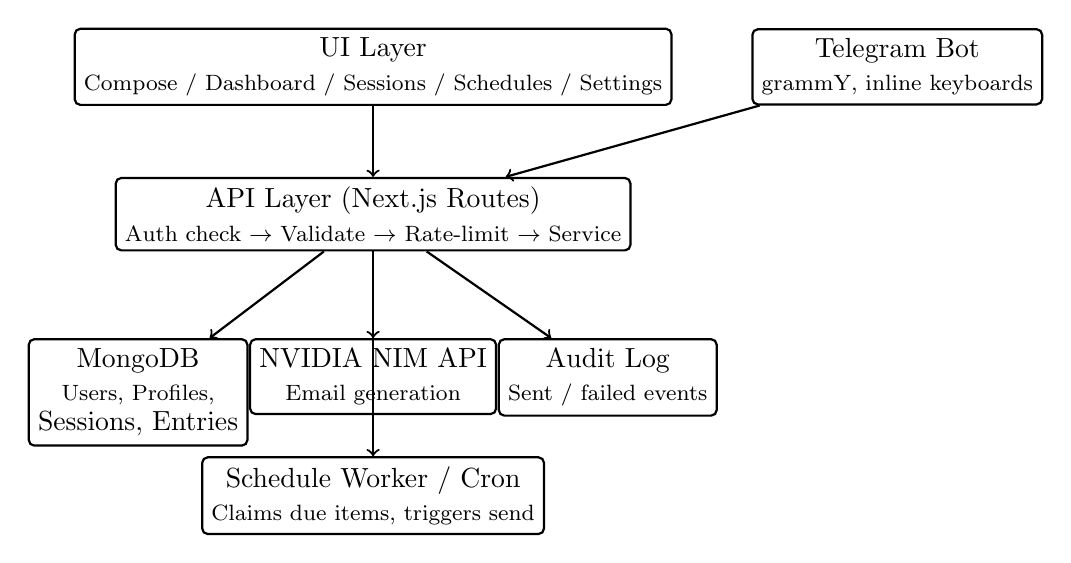
\begin{tikzpicture}[
  node distance=0.9cm,
  every node/.style={draw,thick,minimum height=0.9cm,align=center,font=\fontsize{10}{11}\selectfont},
  box/.style={rectangle,rounded corners=2pt,minimum width=4.6cm,fill=white},
  small/.style={rectangle,rounded corners=2pt,minimum width=2.6cm,fill=white}
]
\node[box] (ui) {UI Layer\\[1pt]\footnotesize Compose / Dashboard / Sessions / Schedules / Settings};
\node[small,right=1.0cm of ui] (tg) {Telegram Bot\\[1pt]\footnotesize grammY, inline keyboards};
\node[box,below=of ui] (api) {API Layer (Next.js Routes)\\[1pt]\footnotesize Auth check $\rightarrow$ Validate $\rightarrow$ Rate-limit $\rightarrow$ Service};
\node[small,below left=1.1cm and -1.7cm of api] (db) {MongoDB\\[1pt]\footnotesize Users, Profiles,\\Sessions, Entries};
\node[small,below=1.1cm of api] (ai) {NVIDIA NIM API\\[1pt]\footnotesize Email generation};
\node[small,below right=1.1cm and -1.7cm of api] (audit) {Audit Log\\[1pt]\footnotesize Sent / failed events};
\node[small,below=2.6cm of api] (sched) {Schedule Worker / Cron\\[1pt]\footnotesize Claims due items, triggers send};

\draw[->,thick] (ui) -- (api);
\draw[->,thick] (tg) -- (api);
\draw[->,thick] (api) -- (db);
\draw[->,thick] (api) -- (ai);
\draw[->,thick] (api) -- (audit);
\draw[->,thick] (api) -- (sched);
\end{tikzpicture}
\caption{Architecture of the Proposed System}
\end{figure}

\begin{table}[h]
\centering
\caption{AI Models Supported}
\begin{tabularx}{\textwidth}{@{}l X X@{}}
\toprule
\textbf{Selector ID} & \textbf{Label} & \textbf{Notes} \\
\midrule
\texttt{deepseek}            & DeepSeek V4 Flash             & Default model; fast, general-purpose drafting. \\
\texttt{nemotron}            & Nemotron Super 49B            & NVIDIA reasoning-tuned model. \\
\texttt{gptOss}              & GPT-OSS 20B                   & Open-weight reasoning model. \\
\texttt{mistralSmall}        & Mistral Small 4 (119B)        & Hybrid instruct/reasoning model. \\
\texttt{llamaMaverick}       & Llama 4 Maverick 17B          & Multimodal mixture-of-experts, 1M context. \\
\texttt{minimaxM27}          & MiniMax M2.7                  & Code/agent-tuned mixture-of-experts model. \\
\texttt{llamaNemotronNano}   & Llama Nemotron Nano 8B VL     & Lightweight multimodal vision-language model. \\
\texttt{nemotron3Ultra}      & Nemotron 3 Ultra 550B         & Flagship reasoning model (550B parameters). \\
\bottomrule
\end{tabularx}
\end{table}

% ======================================================================
% 9. ADVANTAGES OF PROPOSED SYSTEM
% ======================================================================
\section{Advantages of Proposed System}

\begin{itemize}[leftmargin=22pt]
  \item Drafting and sending happen in one application, removing the copy-paste step between a chat tool and a mail client.
  \item The stored profile supplies personal and professional context automatically, instead of it being retyped for every email.
  \item Batch mode turns $N$ repetitive emails into $N$ rows generated and sent from one screen, with status and failure tracking, instead of $N$ separate manual prompts.
  \item Scheduling lets a user prepare a message once and have it delivered automatically at a chosen future date and time, without needing to be present to click Send.
  \item The Gmail credential is encrypted at rest, decrypted only inside the send route, and never returned by any API response -- reducing exposure compared to pasting a password into a general-purpose tool.
  \item Every draft, every send attempt, and every scheduled-email outcome is recorded -- in the session/message history, the schedule detail view, and the audit log respectively -- giving a searchable record that an ad hoc chat-and-copy workflow does not provide.
  \item Eight AI models with different speed, quality, and context-length trade-offs are available from one selector, instead of being limited to a single model's behaviour.
  \item The Telegram bot reuses the same profile, models, and Gmail delivery path as the web application, so a user who links their account gets a genuinely mobile-friendly composition channel without the cost of building and maintaining a separate native app.
\end{itemize}

% ======================================================================
% 10. FEASIBILITY STUDY
% ======================================================================
\section{Feasibility Study} 

\subsection{Technical Feasibility}

All the technology used is freely available and well documented: Next.js and React for the front end and the API layer, MongoDB (an Atlas free-tier cluster or a local instance) for storage, the NVIDIA NIM API for inference, Nodemailer for SMTP delivery through the user's existing Gmail account, and the grammY framework together with the Telegram Bot API for the chat-based composition channel. Deferred delivery is implemented with an in-process, self-unref'd timer for local/self-hosted use and, on serverless deployments such as Vercel, an externally-triggered cron endpoint protected by a shared secret -- both of which are standard, freely available mechanisms that do not require any dedicated job-queue infrastructure. No specialised hardware, paid licence, or institutional infrastructure is required beyond a standard development laptop and an internet connection, and the project team's existing knowledge of JavaScript/TypeScript and REST-style APIs is sufficient to build and maintain the system.

\subsection{Operational Feasibility}

The system does not require a user to change how they send email -- they continue to send from their own Gmail address; AutoCompose only automates the drafting step and, if the user chooses, the sending, scheduled-sending, or Telegram-based sending step. The interface is a standard responsive web page reachable from any modern browser, so no client installation or IT approval is needed before a user can start using it, and a user who additionally wants chat-based access only needs to link an existing Telegram account, which takes under a minute. The only other operational prerequisite is generating a Google App Password once, which takes a few minutes and is explained through an in-app help link. On a Vercel Hobby-tier deployment, per-minute schedule processing is not available (Hobby cron jobs run at most once a day), so timely scheduled delivery in that configuration depends on either a paid Vercel plan or an external cron service calling the processing endpoint every minute; this is noted as a deployment consideration rather than a functional limitation.

\subsection{Economic Feasibility}

Development cost is limited to engineering time: the front end, API layer, and database schema are all built on open-source or free-tier technology (Next.js, MongoDB Atlas free tier, NVIDIA NIM developer access, a free Telegram bot token), so no software licence fee applies. Running cost at small or personal scale is essentially the cost of the MongoDB Atlas tier chosen and any hosting plan used for deployment; AI inference and email delivery (through the user's own Gmail account) do not add direct project cost beyond normal API usage limits, and the Telegram bot itself has no usage fee. 

% ======================================================================
% 11. SOFTWARE ENGINEERING PARADIGM APPLIED
% ======================================================================
\section{Software Engineering Paradigm Applied}

AutoCompose was developed using the \textbf{Incremental Model}. The project began with a minimal but complete vertical slice -- authentication, a single-email compose flow, and AI generation through one model -- and each later increment added one self-contained capability on top of an already-working system: per-user Gmail credentials and direct sending; batch composition and batch sending; automatic recipient extraction from a prompt; file attachments; session-message pagination together with a tone selector; usability refinements such as draft auto-save and collapsible long prompts; a bulk ``Clear All Sessions'' action; a dedicated resume-editing page for correcting AI-parsed resume data; a linked Telegram bot offering a chat-based version of the core compose-and-send flow; and, most recently, an end-to-end email scheduling subsystem with its own database models, API routes, background worker, and UI. The project's own change history records each of these as a separate, dated, independently testable unit of work.

This model was chosen over a single-pass waterfall approach because several requirements were only identified by using an already-working increment -- for example, the need to auto-extract a recipient's email address from the prompt text (Section 14) became apparent only after the basic compose flow was already in active use, the need for a lightweight mobile channel (Section 14.10) became apparent once users started asking to send a quick email without opening a laptop, and the need for scheduled delivery (Section 14.9) became apparent only after batch composition made it common for a user to have several drafted-but-not-yet-sent emails at once -- none of which a fully-specified-upfront approach would have surfaced as naturally. Each increment also kept the system in a demonstrable, working state throughout development, which suited the fixed timeline of a single-semester mini project better than deferring a working build to the very end.

% ======================================================================
% 12. SYSTEM ENVIRONMENT
% ======================================================================
\section{System Environment}

\subsection{Introduction}

The system is built and run entirely on freely available, cross-platform tools. This section lists the languages, frameworks, services, and minimum hardware needed to develop and run AutoCompose.

\subsection{Software Requirements Specification}

\begin{table}[h]
\centering
\caption{Software Requirements}
\begin{tabularx}{\textwidth}{@{}l X@{}}
\toprule
\textbf{Component} & \textbf{Requirement} \\
\midrule
Runtime              & Node.js 22 or later \\
Database             & MongoDB 6 or later (Atlas-hosted or local instance) \\
AI Service           & NVIDIA NIM API key and base URL (cloud inference; no local model hosting needed) \\
Scheduled Delivery    & In-process background worker (local/self-hosted) or an external cron trigger protected by a shared secret (serverless deployments) \\
Chat Access           & A registered Telegram bot token and, on serverless deployments, a webhook secret \\
Package Manager      & npm \\
Version Control      & Git \\
Client (end user)     & Any current evergreen browser (Chrome, Edge, Firefox, or Safari), or the Telegram app for chat-based access \\
\bottomrule
\end{tabularx}
\end{table}

\subsection{Hardware Requirements Specification}

\begin{table}[h]
\centering
\caption{Hardware Requirements}
\begin{tabularx}{\textwidth}{@{}l X@{}}
\toprule
\textbf{Item} & \textbf{Minimum Requirement} \\
\midrule
Processor  &  Dual-core 2.0 GHz or higher \\
RAM        & 2 GB (16 GB recommended for running the dev server and a local MongoDB instance together) \\
Storage                          & 2 GB free space for project dependencies and local data \\
Network                          & Broadband internet connection -- required for MongoDB Atlas, the NVIDIA NIM API, Gmail SMTP, and the Telegram Bot API; the application does not work offline, and scheduled emails can only be processed while the server (or cron trigger) has connectivity \\
Client (end user)                & Any device capable of running a modern web browser, or the Telegram mobile/desktop app \\
\bottomrule
\end{tabularx}
\end{table}

\subsection{Tools, Platforms}

\subsubsection{Front End Tool}
Next.js 16 (App Router), React, TypeScript, TanStack Query for server-state caching, Zustand for client-side UI state, and a custom Neubrutalist CSS design system (no external component framework).

\subsubsection{Back End Tool}
Next.js API routes running on the Node.js runtime, Mongoose as the MongoDB ODM, NextAuth (JWT strategy) for authentication, Zod for request validation, Nodemailer for SMTP delivery, the OpenAI SDK configured against the NVIDIA NIM endpoint for AI generation, the grammY framework for the Telegram bot, and an in-process interval-based worker (with an external cron endpoint as the serverless equivalent) for scheduled-email processing.

\subsubsection{Operating System}
Development is operating-system independent, since the entire stack runs on Node.js (Windows, Linux, or macOS are all suitable).  The deployment target is any hosting platform that supports Node.js 22.

% ======================================================================
% 13. USER CHARACTERISTICS
% ======================================================================
\section{User Characteristics}

AutoCompose is designed for two related but distinct usage patterns.

\textbf{Individual users} -- students and working professionals who occasionally need a single, well-worded email, such as a leave request, a complaint, or a follow-up. They are assumed to have ordinary web-browser literacy and no programming knowledge. The single-compose flow (Section 14.2) and the stored profile (Section 14.5) are designed so this group never has to re-explain their background to the system, the optional scheduling step (Section 14.9) lets them prepare a message ahead of time without needing to remember to send it later, and the Telegram bot (Section 14.10) gives them a way to handle an unexpected email -- a last-minute leave request, for instance -- without opening a laptop.

\textbf{Repeat senders} -- users who regularly send the same kind of email to many different recipients, for example the same recommendation request sent to several referees, or job applications sent to multiple companies. This group is the primary audience for batch mode (Section 14.3), which lets them prepare, generate, and send several personalised drafts from a single screen instead of repeating the single-compose flow once per recipient, and for batch scheduling, which lets them queue an entire batch for delivery at a coordinated future time.

No administrator role exists in the current version of the system; every account sees and manages only its own data, enforced by the ownership rules described in Section 8. No special training is required beyond the in-app hints, such as the Gmail App Password setup link shown in Settings and the account-linking prompt shown when connecting Telegram.

% ======================================================================
% 14. SUMMARY OF SYSTEM FEATURES / FUNCTIONAL REQUIREMENTS
% ======================================================================
\section{Summary of System Features/Functional Requirements}

This section lists the functional requirements implemented in the current version of AutoCompose. Each requirement is described in terms of its inputs, its processing logic, and the output presented to the user.

\subsection{User Registration and Authentication}
\noindent\textbf{Introduction:} Allows a new user to create an account and an existing user to sign in, and keeps the session valid for as long as the user remains logged in.\\
\noindent\textbf{Inputs:} Name and email address (registration); email and password (login).\\
\noindent\textbf{Processing:} Credentials are validated with Zod and checked against the MongoDB \texttt{User} collection; on success, a JWT session is issued by NextAuth. \texttt{requireAuth()} guards every protected API route, and an \texttt{AuthGuard} at the layout level redirects an unauthenticated visitor to the login page. Registration is additionally protected by a per-IP and global rate limit and a hidden honeypot field that silently discards bot submissions.\\
\noindent\textbf{Outputs:} An authenticated session granting access to the Dashboard, Compose, Sessions, Schedules, and Settings pages; an error message on invalid credentials.

\subsection{Single Email Composition}
\noindent\textbf{Introduction:} Generates one professional email draft from a free-text prompt, using a selected AI model, the user's profile, and an optional tone.\\
\noindent\textbf{Inputs:} Prompt text, email category (e.g., leave request, complaint), tone (Formal, Neutral, or Casual -- optional), AI model (optional, defaults to the profile's preferred model), and an optional session ID for continuation.\\
\noindent\textbf{Processing:} The validated request reaches \texttt{POST /api/generate}; the system builds a profile context (signature, formality level, and so on), injects prior conversation history when a session ID is supplied, applies a tone override if one was chosen, and forwards the combined prompt to the selected NVIDIA NIM model. The raw response is split into a subject and a body.\\
\noindent\textbf{Outputs:} A rendered subject and body shown on the Response Display panel; the exchange is saved as a message when it belongs to a session, and a recipient address is auto-extracted from the prompt text when one is present. From this panel the user may immediately send the email, or add it to a schedule for later delivery (Section 14.9).

\subsection{Batch Email Composition and Generation}
\noindent\textbf{Introduction:} Creates and AI-generates multiple personalised email drafts inside one batch session, for sending similar correspondence to different recipients.\\
\noindent\textbf{Inputs:} Number of rows to add (1 to 50), and, per row, a category, a prompt, and a recipient address; an optional shared AI model selection; optional shared or per-row file attachments.\\
\noindent\textbf{Processing:} Each row is created as a \texttt{BulkEntry} record in the \texttt{pending} state. A row can be generated individually, or several rows can be re-categorised together; generation is rate-limited and tracked through six states (\texttt{pending} $\rightarrow$ \texttt{generating} $\rightarrow$ \texttt{generated}/\texttt{failed} $\rightarrow$ \texttt{sending} $\rightarrow$ \texttt{sent}). The interface polls every two seconds while any row is mid-generation or mid-send.\\
\noindent\textbf{Outputs:} A per-row generated subject and body with a status badge, and an aggregate count of ready, sent, failed, and pending rows on the toolbar. Generated rows can be sent individually, sent as a group with automatic rate-limit-aware pacing, or added to a schedule for deferred delivery as a batch (Section 14.9).

\subsection{Session History and Management}
\noindent\textbf{Introduction:} Stores and organises every composed conversation, single or batch, so it can be reviewed, renamed, archived, or removed later.\\
\noindent\textbf{Inputs:} A session title (auto-generated or user-defined), a search keyword, an archive toggle, a per-session delete action, and a bulk ``Clear All Sessions'' action.\\
\noindent\textbf{Processing:} Sessions are listed with infinite-scroll pagination and full-text search on the title. A rename is applied optimistically, with a rollback if the request fails. Deleting a session performs a soft delete (the \texttt{isDeleted} flag is set) rather than a permanent removal; the ``Clear All Sessions'' action performs the same soft delete across every active session for the user in one confirmed operation. Messages inside a session load in pages of 20, newest first, with a ``Load earlier messages'' control, and long user prompts collapse automatically with a ``Show full prompt'' toggle.\\
\noindent\textbf{Outputs:} A searchable, paginated list of sessions carrying Single/Batch badges; the full message thread for a selected session; a ``Draft restored'' banner when the user returns to an unfinished compose form.

\subsection{Profile and Preference Management}
\noindent\textbf{Introduction:} Maintains the personal, professional, writing-style, and job-application information used to personalise every AI generation, together with the user's default AI model.\\
\noindent\textbf{Inputs:} Personal details (name, phone, location); professional details (designation, organisation); writing preferences (formality level, tone, signature, language); job-application links (resume URL, LinkedIn, GitHub, portfolio); preferred AI model; Gmail delivery credentials (Section 14.6).\\
\noindent\textbf{Processing:} Each settings section is validated and saved independently through \texttt{PATCH /api/profile}. The preferred model becomes the default selection on the Compose and Resume forms, but does not retroactively change a form that is already open.\\
\noindent\textbf{Outputs:} The updated profile is reflected in the next AI generation; the default model and tone are pre-filled the next time Compose is opened.

\subsection{Saved Contacts}
\noindent\textbf{Introduction:} Lets a user store frequently-used name-and-email pairs and pick them while filling the recipient field anywhere in the application.\\
\noindent\textbf{Inputs:} A name and an email address, added individually through the Contacts section in Settings; or an edit or deletion of an existing contact.\\
\noindent\textbf{Processing:} Each contact is validated (name between 1 and 100 characters, valid email address) and saved to the \texttt{Profile.contacts} array as an object with a \texttt{id}, \texttt{name}, and \texttt{email} field, with an overall limit of 500 contacts per user. Every recipient input on the compose page, the session message bubble, the batch entry row, and the send-email dialog now uses a shared \texttt{ContactAutocomplete} component instead of a plain \texttt{<input type="email">}: as the user types, the component filters saved contacts by case-insensitive substring match on either the name or the email (up to 5 suggestions), supports arrow-key navigation, Enter to select, and Escape to close, and fills the field with the chosen email address.\\
\noindent\textbf{Outputs:} A saved contact appears in the autocomplete list when the user types a matching string into any recipient field; the field is populated with the selected email address.

\subsection{Secure Email Delivery via Gmail}
\noindent\textbf{Introduction:} Sends a finished draft from the user's own Gmail account using an application-specific password, without ever returning that password to the client.\\
\noindent\textbf{Inputs:} Recipient address, subject, and body (editable in the Send dialog); optional file attachments (up to 10 MB per file, 24 MB total, 20 files); a one-time Gmail address and 16-character App Password configured under Settings.\\
\noindent\textbf{Processing:} The App Password is encrypted at rest using AES-256-GCM envelope encryption: each user's password is encrypted under a per-user data encryption key (DEK), and that DEK is itself encrypted under a key derived from \texttt{AUTH\_SECRET}, so compromising \texttt{AUTH\_SECRET} alone does not expose any user's plaintext credential; the password is decrypted only inside the send-email route. A fresh SMTP connection to \texttt{smtp.gmail.com:465} is opened per send and closed immediately afterwards, with any attachments forwarded to the transporter. Sending is rate-limited to 5 requests per 60 seconds per user, and every attempt is written to the audit log without the password.\\
\noindent\textbf{Outputs:} The email is delivered from the user's own address; the dialog reports success or a specific failure (\texttt{CREDENTIALS\_NOT\_CONFIGURED}, \texttt{CREDENTIALS\_INVALID}, \texttt{SEND\_FAILED}, or \texttt{RATE\_LIMIT}).

\subsection{Resume Parsing and Profile Enrichment}
\noindent\textbf{Introduction:} Extracts structured information from an uploaded resume to enrich the user's profile, allows the user to review and correct that extracted data, and improves job-application-related email generation.\\
\noindent\textbf{Inputs:} A resume file (PDF, DOCX, or TXT) and an AI model for parsing (defaults to DeepSeek); on the dedicated resume-editing page, manual corrections to contact information, links (LinkedIn, GitHub, portfolio), skills, education, experience, and projects.\\
\noindent\textbf{Processing:} The file is streamed to \texttt{POST /api/profile/resume}, parsed by the selected model into skills, education, experience, and projects, and saved to \texttt{Profile.resume}. The raw extracted text is kept internally for parsing accuracy but withheld from every \texttt{GET} response. The user may then open the \texttt{/settings/resume/edit} page, where a modular editor form tracks unsaved changes and prompts before navigation away, and saves corrections back through \texttt{PATCH /api/profile/resume}.\\
\noindent\textbf{Outputs:} A structured resume summary shown in Settings, editable in full on the resume-editing page; the model used for parsing is recorded for audit and made available to future job-application prompts.

\subsection{Audit Logging}
\noindent\textbf{Introduction:} Keeps a record of security- and delivery-relevant actions for accountability and troubleshooting.\\
\noindent\textbf{Inputs:} System-generated events, such as an email being sent or failing to send, credentials being saved or removed, a scheduled email being sent or failing, or a Telegram account being linked or unlinked.\\
\noindent\textbf{Processing:} Each action is written to the \texttt{AuditLog} collection with the actor, the affected entity, contextual metadata, IP address (where applicable), and user agent -- but never with any secret value; the App Password and Telegram login codes are excluded from every log entry by design.\\
\noindent\textbf{Outputs:} A queryable audit trail that can be used to confirm what was sent, when, and by whom, and to diagnose a delivery, scheduling, or Telegram-linking failure without exposing any credential.

\subsection{Email Scheduling}
\noindent\textbf{Introduction:} Defers the delivery of a drafted email -- generated individually or as part of a batch -- to a future date and time chosen by the user, with full timezone support, instead of requiring the user to send it manually at that moment.\\
\noindent\textbf{Inputs:} A schedule name, a target date and time, and the browser's timezone (when creating a schedule); one or more emails added to a schedule from the single-compose success panel, from a past session message, or from a batch of generated entries; edits to a not-yet-sent scheduled email's recipient, subject, or body; a cancel action on an active schedule; a retry action on a failed item.\\
\noindent\textbf{Processing:} A schedule is stored as a \texttt{Schedule} document with status \texttt{active}, and each email added to it is stored as a \texttt{ScheduledEmail} item. A single-sourced item snapshots its recipient, subject, and body at scheduling time; a batch-sourced item instead stores a reference to its originating batch entry and is marked \texttt{awaiting\_content}, so that its content is generated by the AI provider only at send time. Unique sparse indexes on the source message and source batch-entry references prevent the same draft from being added to a schedule twice; duplicates are silently skipped and reported to the user. A background process -- an in-process worker ticking once a minute in local/self-hosted deployments, or an external cron call to a secret-protected endpoint on serverless deployments -- finds schedules whose time has arrived, atomically claims a batch of their due items, generates content for any \texttt{awaiting\_content} items, sends each item through the same Gmail SMTP path used for immediate sending, and marks each item \texttt{sent} or \texttt{failed}. Once all items in a schedule have been processed, the schedule itself is marked \texttt{sent}, or \texttt{expired} if its time passed with items still unprocessed. A user may also cancel an active schedule at any time, or manually trigger processing of a single schedule for testing.\\
\noindent\textbf{Outputs:} A list of the user's schedules with status and countdown information; a schedule detail page showing every email item with its delivery state, with retry and remove actions available on items that have not yet been sent; confirmation when an email is successfully added to, or already present in, a schedule; and, once due, the same delivered-email outcome as an immediate send, recorded in the audit log as a schedule-specific event.

\subsection{Telegram Bot Integration}
\noindent\textbf{Introduction:} Gives a linked user a chat-based alternative to the web Compose page, so a single email can be described, generated, reviewed, and sent entirely from Telegram, using the same profile, AI models, and Gmail delivery path as the rest of the system.\\
\noindent\textbf{Inputs:} A one-time account-linking action started from Settings; the bot commands \texttt{/start}, \texttt{/menu}, \texttt{/compose}, \texttt{/cancel}, \texttt{/help}, and \texttt{/status}; a category chosen from an inline keyboard; a free-text description of the email; and, when sending, a recipient address (or a ``Send to me'' shortcut using the user's own Gmail address) and an optional custom subject.\\
\noindent\textbf{Processing:} Linking is a short handshake: the web app generates a random, bcrypt-hashed code with a ten-minute expiry and a deep link into Telegram; opening that link triggers the bot's \texttt{/start} handler, which verifies the code against every user with a still-valid code and, on a match, stores the chat ID against that account. Once linked, \texttt{/compose} walks the user through a small state machine -- selecting a category, describing the email, generating a draft through the same AI provider used by the web app, and reviewing it with Send / Send to me / Regenerate / Menu options -- before dispatching through the identical encrypted-credential Gmail SMTP path used by web and batch sending. Conversation state is stored per chat with a 24-hour TTL and a version number for optimistic-concurrency protection against out-of-order Telegram updates, and every incoming webhook update is checked against a short-lived idempotency record so a duplicate delivery from Telegram cannot generate or send the same email twice. The webhook itself only accepts requests carrying the correct shared secret header. Account linking, sends, and login-code generation are each separately rate-limited per user.\\
\noindent\textbf{Outputs:} A generated email reviewed and sent (or discarded) inside the same Telegram chat, with success or a specific failure reported back through the bot; a linked-status indicator and unlink option shown under Settings; and the same audit-log coverage -- linked, unlinked, message received, command executed, email generated, email sent, and email send failed -- as the equivalent web actions.

\end{document}